\mainmatter%
\setcounter{page}{1}

\lectureseries[\course]{\course}

\auth[\lecAuth]{Lecturer: \lecAuth\\ Scribe: \scribe}
\date{November 19, 2009}

\setaddress%

% the following hack starts the lecture numbering at 15
\setcounter{lecture}{14}
\setcounter{chapter}{14}

\lecture{Numerical Methods}

\section{Exit Problem Review}
In Lecture 14 we looked at exit problems where the system dynamics and initial conditions were given by
\begin{align*}
\dot{\xi} &= f(\xi,u) = g(\xi,k(\xi),u) \\
\xi_0 &= x
\end{align*}
Here, $u$ represents a disturbance and $k(\xi)$ is the control.
The cost function was
$$J(x,u) = \int_0^T\rho+\frac{1}{2}|u_t|^2dt$$
which led to the dynamics being $\dot{\xi}=u_t$.
The idea was to use the value function
$$V(x) = \inf_{u\in\mathcal{U}_0^\ast}J(x,u)$$
If that is the value function for all $u\in\mathcal{U}_0^\ast$ then we get
$$V(x) = \int_0^\tau \rho + \frac{1}{2}|u_t|^2dt = \tau\left[\rho+\frac{1}{2}\int_0^\tau|u_t|^2dt\right]$$
This leads to
$$\tau\geq\frac{V(x)}{\rho+\frac{1}{2\tau}\int_0^\tau|u_t|^2dt}$$
If we then fix $\mathbb{P}<\infty$ and let
$$\tilde{\mathcal{U}}^\mathbb{P} = \left\lbrace u\in\mathcal{U}_0^\ast~|~\frac{1}{T}\int_0^T|u_t|^2dt \leq \mathbb{P}~\forall T<\infty \right\rbrace$$
we get an expression for $\tau$ such that
$$\tau\geq \frac{V(x)}{\rho+\frac{\mathbb{P}}{2}}$$
This is a robustness statement for the controller.

\section{Numerical Methods}
There are three main classes of solving these problems using numerical methods.
\begin{itemize}
\item Characteristics.
This is similar to Pontryagin's optimality principle.
It is only really good for deterministic and pseudo-spectral systems.
\item Finite element or grid-based methods.
These are used to solve the HJB or HJI (Hamilton-Jacobi-Isaacs) PDEs.
These methods typically require viscocity solutions and are good for low dimensional, high complexity dynamics systems.
\item Max-plus or idempotent methods.
These are good for high dimensional, low complexity dynamics systems.
\end{itemize}
The last two methods are useful in deterministic, stochastic and game-type problems.

\section{Characteristics for Exit Problem}
We want to solve
\begin{align*}
0 &= f(x,\nw(x)), x\in G \\
W(x) &= 0, x\in\partial G
\end{align*}

Figure~\ref{fig:15g} shows some of the state space.
For notation in the rest of this lecture we will let functions be of the form $f(x,p)$, where the first argument is $x$ and the second argument is $p$.
Then we have
$${[\nabla_p f(x,p)]}_i = f_{p_i}(x,p)$$

\begin{figure}[ht!]
\centering
\includegraphics[width=.4\textwidth]{images/15g}
\caption{The space $G$ showing possible trajectories $\eta_r$ starting at $\bar{x}$.}
\label{fig:15g}
\end{figure}

Our goal is to find $W$.
We start by letting $z_r=W(\eta_r)$ so that $z_0=W(\eta_0)=W(\bar{x})$.
Then we get
$$\dot{z}_r = \sum_{i=1}^n W_{x_i}(\eta_r){[\dot{\eta}_r]}_i = \nw(\eta_r)\cdot \dot{\eta}_r$$
Let $\vp_r=\nw(\eta_r)$.
This leads to $\dot{z}_r=\vp_r\dot{\eta}_r$.
From here we choose to let
$$\dot{\eta}_r = \nabla_p f(\eta_r,\nw(\eta_r)) = \nabla_p f(\eta_r,\vp_r)$$

Now, looking at the dynamics of the co-state we see that
\begin{align}
\label{eq:15vp}
\dot{\vp}_r &= \frac{d}{dr}[\nw(\eta_r)] \nonumber \\
\Rightarrow {[\dot{\vp}_r]}_i &= \frac{d}{dr}[W_{x_i}(\eta_r)] \nonumber \\
&= \sum_{j=1}^n W_{x_i x_j}(\eta_r){[\dot{\eta}_r]}_j \nonumber \\
&= \sum_{j=1}^n W_{x_i x_j}(\eta_r)f_{p_j}(\eta_r,\vp_r)
\end{align}
This is what the dynamics of $\vp$ need to be given our choice of $\dot{\eta}_r$ above.
We still need to find $W_{x_i x_j}$.
But, since
$$f(x,\nw(x)) = 0~\forall x\in G$$
we have that
\begin{align}
\label{eq:15fxi}
0 &= \frac{\partial}{\partial x_i}[f(x,\nw(x))] \nonumber \\% chktex 9
&= f_{x_i}(x,\nw(x)) + \sum_{j=1}^n f_{p_j}(x,\nw(x))W_{x_j x_i}(x)
\end{align}
By (\ref{eq:15vp}) and (\ref{eq:15fxi}) we get
\begin{align*}
{[\dot{\vp}_r]}_i &= -f_{x_i}(\eta_r,\vp_r) \\
\Rightarrow \dot{\vp} &= -\nabla_x f(\eta_r,\vp_r)
\end{align*}
This lets us keep track of $\eta$ as we iterate.

Recapping, now we know
\begin{align*}
\dot{\eta}_r &= \nabla_p f(\eta_r,\vp_r) \\
\dot{\vp}_r &= -\nabla_x f(\eta_r,\vp_r) \\
\dot{z}_r &= \vp_r\dot{\eta}_r = \vp_r\cdot \nabla_p f(\eta_r,\vp_r)
\end{align*}
These three equations are $2n+1$-dimensional.
We want to track the trajectory in from the boundary so we use
\begin{align*}
\eta_0 &= \bar{x} \in \partial G \\
z_0 &= W(\eta_0) = \psi(\eta_0) = \psi(\bar{x}) \\
\vp_0 &= \nw(\bar{x})
\end{align*}
But, we still don't know $W$ because that is what we are trying to solve for!

Looking at the boundary, as in Figure~\ref{fig:15gboundary}, we know
$$f(\bar{x},\nw(\bar{x})) = f(\bar{x},\vp_0) = 0$$
This is only a single equation but we have that $\vp$ is $n$-dimensional.
Let $\bar{u}$ be the outward normal at $\bar{x}$.
For this to work we need the boundary $\partial G$ to be smooth because we are also using $W\in C^2(G)$, or second derivatives.
Let $\nu$ be the hypertangent plane.
Because the boundary is smooth we know that the directional derivatives in $\nu$ must match and we get
\begin{align*}
W_\nu(\bar{x}) &= \psi_\nu(\bar{x}) \\
\nw(\bar{x})\cdot \nu &= \psi_\nu(\bar{x})
\end{align*}
Now, we also know that there exists $\nu_1,\nu_2,\ldots,\nu_{n-1}$ that span the hyperplane.
Using this it is sufficient to have
$$\nw(\bar{x})\cdot\nu_i = \psi_{\nu_i}(\bar{x})~\forall i\in\]1,n-1\[$$
This leads to
\begin{align*}
&\vp_0\cdot\nu_i = \psi_{\nu_i}(\bar{x}) \\
&f(\bar{x},\vp_0) = 0
\end{align*}
This gives us $n$ equations in $n-1$ dimensions and we can solve the problem.

\begin{figure}[ht!]
\centering
\includegraphics[width=.4\textwidth]{images/15gboundary}
\caption{A close-up look at the boundary of the space $G$.}
\label{fig:15gboundary}
\end{figure}

\subsection{Remarks}
\begin{itemize}
\item We used $W\in C^2(G)$ and $\partial G$ smooth.
\item These are necessary but not sufficient conditions for computing a solution.
\item $\eta_r$ may not cover all of $G$, i.e., we may not have trajectories that reach all of the state space.
\item $\eta_r$ may cross.
      Once the trajectories cross it may not yield the true solution anymore.
      This results in a bookkeeping nightmare.
\end{itemize}

\begin{example}
We are taking a characteristic approach to Example~\ref{ex:14exit}.
We start with
\begin{align*}
0 = \rho - \frac{1}{2}|\nw(x)|^2 = f(x,\nw(x))&, \qquad |x|<R \\
W(x) = 0&, \qquad |x| = R
\end{align*}
We also have that
\begin{align*}
f(x,p) &= \rho-\frac{1}{2}|p|^2 \\
\dot{\eta}_r &= \nabla_p f(\eta_r,\vp_r) = -\vp_r \\
\dot{\vp}_r &= -\nabla_x f(\eta_r,\vp_r) = 0 \\
\dot{z}_r &= \vp_r\cdot\dot{\eta}_r = \vp_r\cdot(-\vp_r) = -|\vp_r|^2
\end{align*}
The boundary conditions are
\begin{align*}
\eta_0 = x, \qquad z_0=0, \qquad |x|=R
\end{align*}
This leads to
\begin{align}
\label{eq:15vpr}
0 &= f(\eta_0,\vp_0) = \rho-\frac{1}{2}|\vp_0|^2 \nonumber \\
|\vp_0| &= \sqrt{2\rho} \nonumber \\
|\vp_r| &= \sqrt{2\rho}~\forall r
\end{align}
From Figure~\ref{fig:15circlezoom} we see that
\begin{align}
\label{eq:15vpo}
&\vp_0\cdot\nu = \psi_\nu(\bar{x}) \nonumber \\
&\frac{1}{R}\vp_0\cdot\left(\begin{array}{c} -x_2 \\ x_1 \end{array}\right) = 0 \nonumber\\
&\vp_{0_1} (-x_2) + \vp_{0_2}x_1 = 0 \nonumber\\
&\vp_{0_1}x_2 = \vp_{0_2}x_1
\end{align}

\begin{figure}[ht!]
\centering
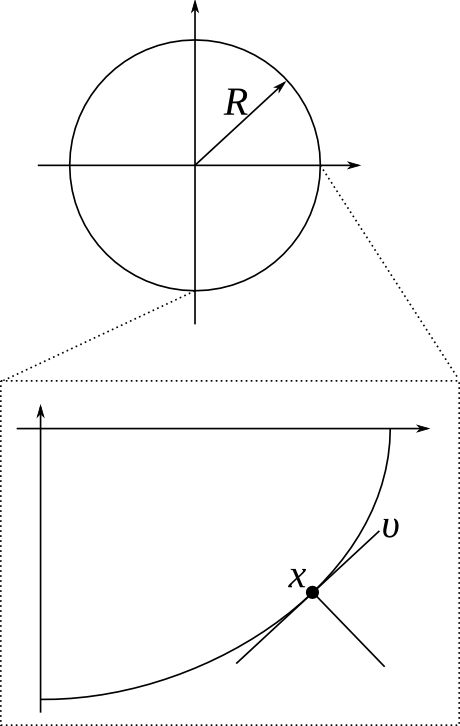
\includegraphics[width=.4\textwidth]{images/15circlezoom}
\caption{A close-up look at the boundary of the space.}
\label{fig:15circlezoom}
\end{figure}

By (\ref{eq:15vpr}) and (\ref{eq:15vpo}) we get
$$\vp_0 = \pm\frac{\sqrt{2\rho}}{R}\cdot\left(\begin{array}{c} -x_2 \\ x_1 \end{array}\right) = \pm\frac{\sqrt{2\rho}}{R}x$$
Then, because $\vp_r$ is constant, we get
$$\vp_r = \frac{\sqrt{2\rho}}{R}x~\forall~r$$
and
\begin{align*}
\dot{\eta}_r &= \mp \frac{\sqrt{2\rho}}{R}x~\forall r \\
\eta_0 &= x \\
\eta_r &= x\mp\frac{\sqrt{2\rho}}{R}xr = \left(1\mp\frac{\sqrt{2\rho}r}{R}\right)x
\end{align*}
We want to have $\eta_r\in G$ for $r>0$ so
$$\eta_r = \left(1-\frac{\sqrt{2\rho}r}{R}\right)x$$
From Figure~\ref{fig:15traj} we want
\begin{align*}
y &= \eta_r = \left(1-\frac{\sqrt{2\rho}r}{R}\right)x \\
|y| &= \left(1-\frac{\sqrt{2\rho}r}{R}\right)|x| \\
&= \left(1-\frac{\sqrt{2\rho}r}{R}\right)R \\
&= R-\sqrt{2\rho}r \\
r &= \frac{R-|y|}{\sqrt{2\rho}}
\end{align*}

\begin{figure}[ht!]
\centering
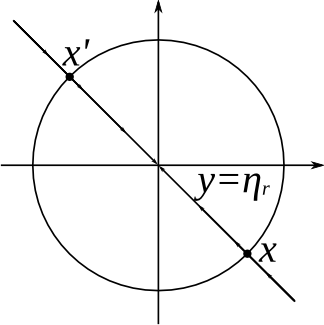
\includegraphics[width=.4\textwidth]{images/15traj}
\caption{Possible trajectories in the space.}
\label{fig:15traj}
\end{figure}

This leads to
\begin{align*}
\dot{z}_r &= \vp\cdot\dot{\eta}_r = -|\vp_r|^2 = -2\rho \\
z_0 &= 0 \\
z_r &= -2\rho r
\end{align*}
And finally we are able to compute $W$ as
\begin{align*}
\boxed{W(y) = z_r = -2\rho r = -2\rho\left(\frac{R-|y|}{\sqrt{2\rho}}\right) = -\sqrt{2\rho}(R-|y|)}
\end{align*}
Note that there is likely a sign error somewhere in this example.
It is a solution but the wrong solution.
Typically there are two solutions possible for these problems with solution spaces that look like a cone and an inverted cone as in Figure~\ref{fig:15solcone}.
One of the cones represents the true solutions and the other cone the false solutions.
$\lozenge$
\end{example}

\begin{figure}[ht!]
\centering
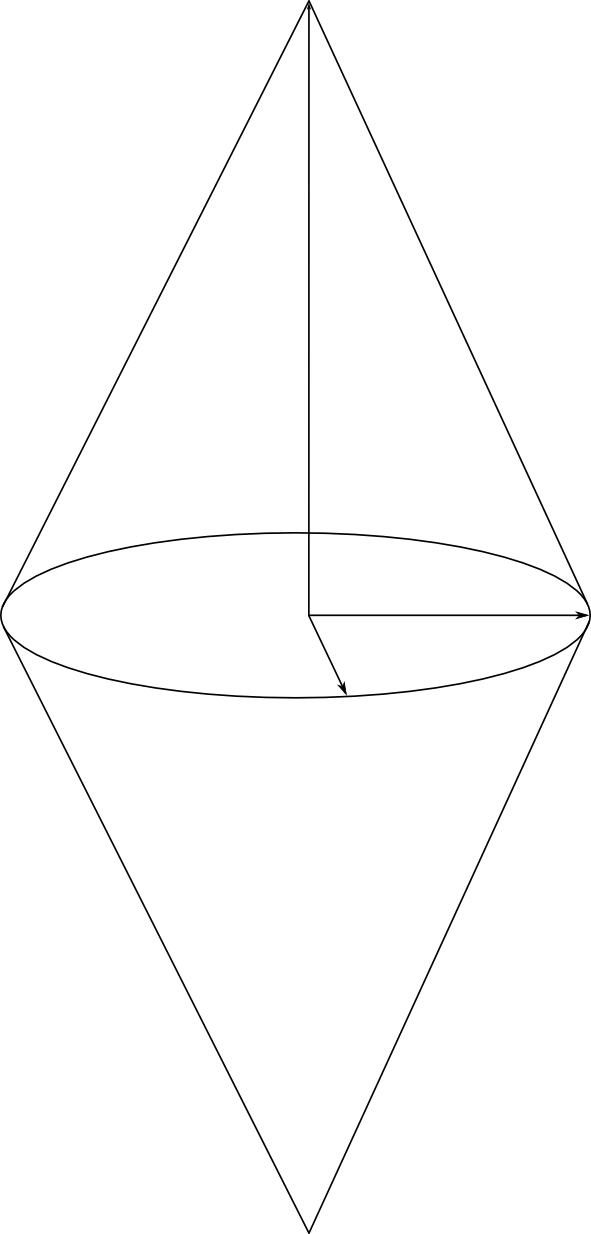
\includegraphics[width=.25\textwidth]{images/15solcone}
\caption{Dual cones showing possible solution spaces.}
\label{fig:15solcone}
\end{figure}% chktex 17
